% ======================================================================
% BLOQUE 1 — El universo temprano, el CMB y QUBIC
% ======================================================================
\section{Universo temprano y QUBIC}
\bloque{COSMOLOGÍA}

% ---------------------------------------------------------------- 3
\begin{frame}{Un universo que se enfría al expandirse}
  \begin{columns}[c,onlytextwidth]
    \column{0.64\textwidth}
    \begin{tikzpicture}
      \begin{loglogaxis}[coloquio, width=\linewidth, height=6.0cm,
        xmin=1e-12, xmax=3e18, ymin=0.1, ymax=1e17,
        xlabel={tiempo desde el Big Bang [s]},
        ylabel={temperatura de la radiación [K]},
        xtick={1e-12,1e-8,1e-4,1,1e4,1e8,1e12,1e16},
        ytick={1,1e4,1e8,1e12,1e16}, grid=major]
        \addplot[very thick, itedaTeal, mark=none] coordinates {
          (1e-12,4.7e15) (1e-11,1.5e15) (2e-5,1.8e12) (1,1e10) (180,8e8)
          (1.6e12,9.3e3) (1.2e13,2970) (2.2e16,23.7) (4.35e17,2.7255)};
        \addplot[only marks, mark=*, mark size=2.3pt, itedaOrange] coordinates {
          (1e-11,1.5e15) (2e-5,1.8e12) (180,8e8) (1.2e13,2970) (4.35e17,2.7255)};
        \node[etiqueta, anchor=south west] at (axis cs:2e-11,1.6e15)
          {\scriptsize ruptura electrodébil ($10^{-11}$\,s)};
        \node[etiqueta, anchor=south west] at (axis cs:4e-5,1.9e12)
          {\scriptsize se forman protones y neutrones};
        \node[etiqueta, anchor=south west] at (axis cs:400,8e8)
          {\scriptsize nucleosíntesis: H, He};
        \draw[itedaOrange, thick] (axis cs:1.2e13,2970) -- (axis cs:1e8,1e5);
        \node[font=\scriptsize\bfseries, text=itedaOrange, anchor=east, align=right]
          at (axis cs:1e8,1e5) {CMB: 380.000 años, $\approx$3000\,K};
        \draw[itedaTealDark, thick] (axis cs:4.35e17,2.7255) -- (axis cs:1e9,3);
        \node[font=\scriptsize\bfseries, text=itedaTealDark, anchor=east, fill=white, inner sep=1pt]
          at (axis cs:1e9,3) {hoy: 2,7\,K, 13.800 millones de años};
      \end{loglogaxis}
    \end{tikzpicture}
    \column{0.33\textwidth}
      \small
      La expansión \textbf{estira la longitud de onda} de cada fotón: la
      radiación se enfría como la inversa del tamaño del universo.
      \vspace{2pt}
      \begin{clave}
        Hasta los 380.000 años, materia y luz están en equilibrio: es la
        temperatura \textbf{de todo}. Después, es la de los fotones del CMB.
      \end{clave}
      \vspace{4pt}

      \esquematico\\[-1pt]{\tiny\color{itedaGray} órdenes de magnitud}
  \end{columns}
\end{frame}

% ---------------------------------------------------------------- 4
\begin{frame}{Un plasma opaco}
  \begin{columns}[T,onlytextwidth]
    \column{0.58\textwidth}
    \vspace{4pt}
    \begin{tikzpicture}[x=1cm,y=1cm]
      \begin{scope}
        \fill[itedaOrange!12, rounded corners=3pt] (0,0) rectangle (3.7,3.4);
        \pgfmathsetseed{11}
        \foreach \i in {1,...,32}{
          \pgfmathsetmacro{\px}{0.2+3.3*rnd}\pgfmathsetmacro{\py}{0.2+3.0*rnd}
          \fill[cmbAzul] (\px,\py) circle (1.3pt);}
        \foreach \i in {1,...,28}{
          \pgfmathsetmacro{\px}{0.2+3.3*rnd}\pgfmathsetmacro{\py}{0.2+3.0*rnd}
          \fill[cmbRojo] (\px,\py) circle (2.0pt);}
        \draw[itedaOrange, very thick, -{Stealth}, rounded corners=1pt]
          (0.3,1.8) -- (0.85,2.4) -- (1.15,1.5) -- (1.8,1.9) -- (1.5,2.85)
          -- (2.35,3.0) -- (2.6,2.0) -- (2.05,1.1) -- (2.9,0.7) -- (3.25,1.6);
        \node[font=\small\bfseries, anchor=south, align=center] at (1.85,3.45)
          {antes de 380.000 años};
        \node[font=\scriptsize, text=itedaGray, anchor=north, align=center] at (1.85,-0.05)
          {plasma de $e^-$ y núcleos:\\el fotón rebota sin parar};
      \end{scope}
      \begin{scope}[xshift=4.1cm]
        \fill[cmbAzul!10, rounded corners=3pt] (0,0) rectangle (3.7,3.4);
        \pgfmathsetseed{5}
        \foreach \i in {1,...,24}{
          \pgfmathsetmacro{\px}{0.25+3.2*rnd}\pgfmathsetmacro{\py}{0.25+2.9*rnd}
          \draw[cmbAzul!70] (\px,\py) circle (3.2pt);
          \fill[cmbRojo] (\px,\py) circle (1.4pt);}
        \draw[foton, itedaOrange, very thick] (0.2,2.8) -- (3.6,2.8);
        \draw[foton, itedaOrange, very thick] (0.2,1.7) -- (3.6,1.7);
        \draw[foton, itedaOrange, very thick] (0.2,0.6) -- (3.6,0.6);
        \node[font=\small\bfseries, anchor=south] at (1.85,3.45)
          {después};
        \node[font=\scriptsize, text=itedaGray, anchor=north, align=center] at (1.85,-0.05)
          {átomos neutros:\\el fotón viaja libre hasta hoy};
      \end{scope}
      \node[font=\scriptsize, anchor=west] at (0,-1.0) {\textcolor{cmbAzul}{$\bullet$} electrón
        \quad \textcolor{cmbRojo}{$\bullet$} protón \quad
        \textcolor{cmbAzul!70}{$\circ$} átomo de hidrógeno};
    \end{tikzpicture}
    \column{0.39\textwidth}
      \small
      Los fotones chocan con los electrones libres:\\[4pt]
      \cifra{$\sim$5.000 años luz}{camino libre medio de un fotón\\poco antes de los 380.000 años}\\[4pt]
      \cifra{$\sim$600.000 años luz}{tamaño del universo observable entonces}\\[4pt]
      \begin{clave}
        A $\sim$3000\,K se forman átomos y los fotones \textbf{se desacoplan}:
        lo más lejos que podemos ver con luz.
      \end{clave}
  \end{columns}
\end{frame}

% ---------------------------------------------------------------- 5
\begin{frame}[plain]
  \begin{tikzpicture}[remember picture, overlay]
    \fill[noche] (current page.south west) rectangle (current page.north east);
    \node[inner sep=0pt] at ([yshift=-0.1cm]current page.center)
      {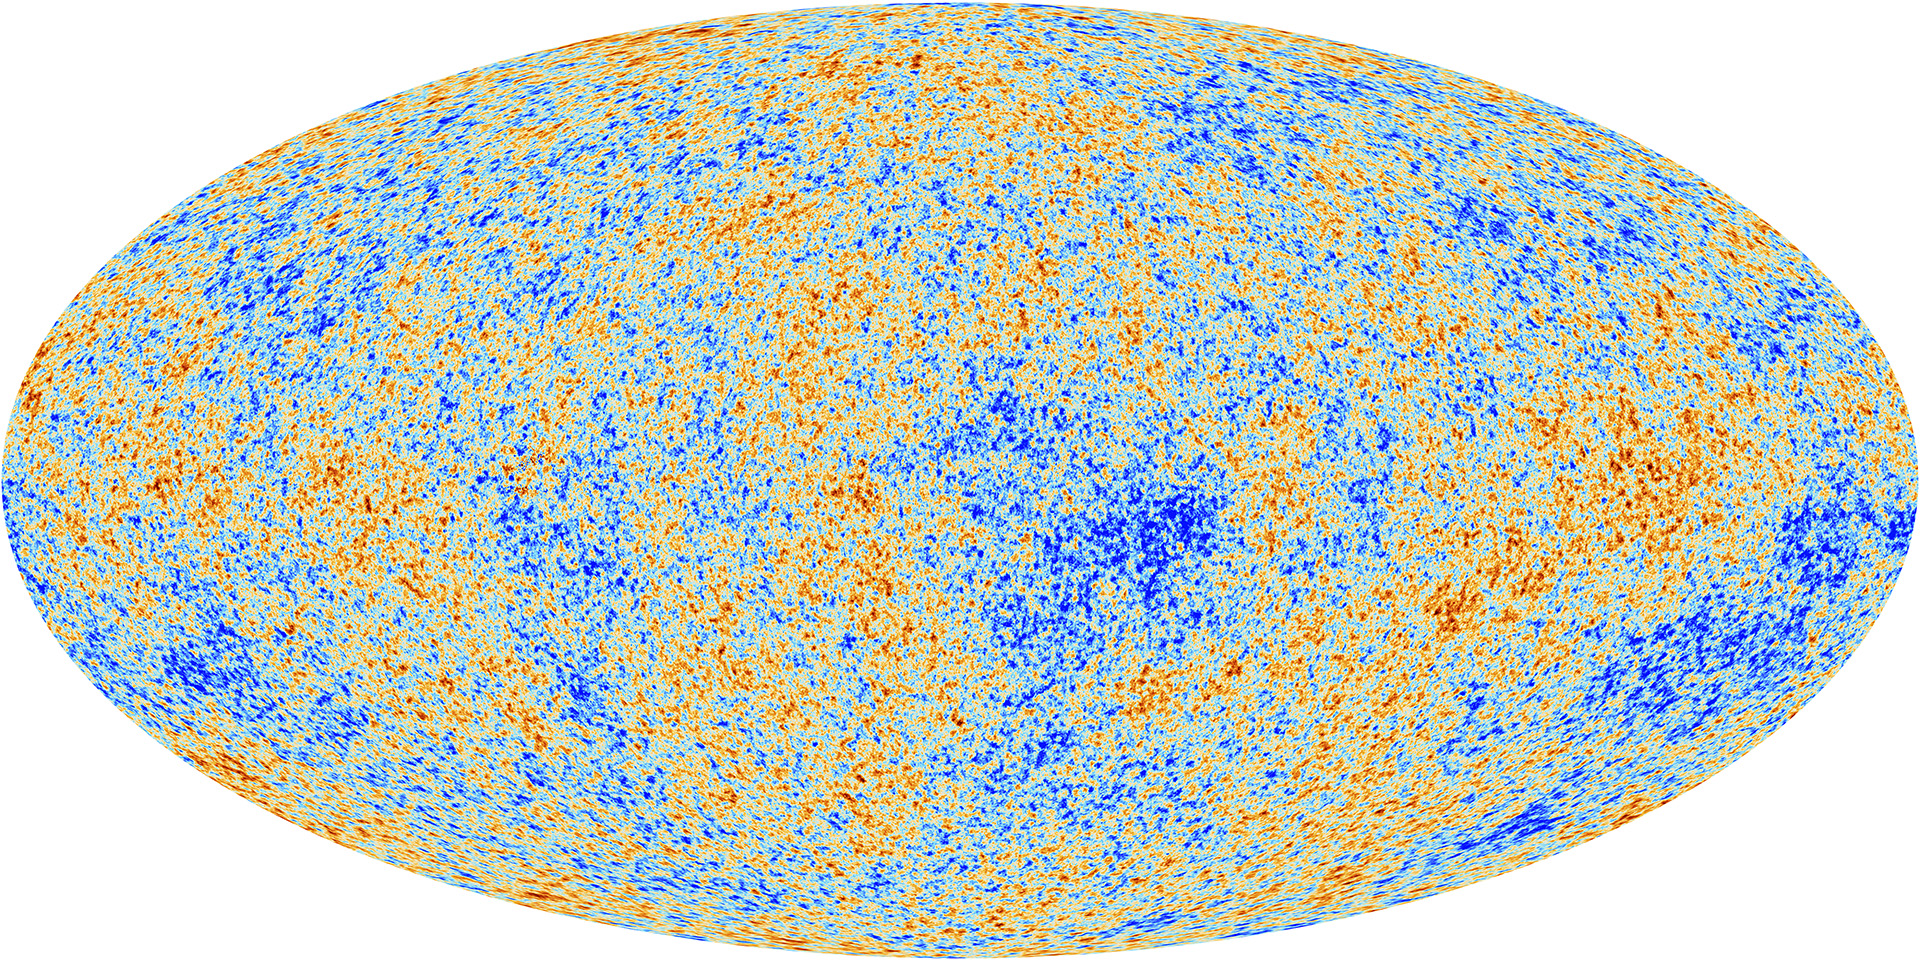
\includegraphics[width=0.78\paperwidth]{externas/planck_cmb_2013.jpg}};
    \node[anchor=north west, text=white, font=\Large\bfseries]
      at ([xshift=0.6cm, yshift=-0.35cm]current page.north west)
      {La fotografía más antigua del universo};
    \node[anchor=south, text=white, font=\small]
      at ([yshift=0.42cm]current page.south)
      {$T_0 = 2{,}7255$\,K \quad · \quad
       \textcolor{itedaOrange}{manchas de $\pm$1 parte en 100.000} \quad · \quad
       380.000 años post Big Bang};
  \end{tikzpicture}
  \creditoblanco{ESA y Colaboración Planck (2013)}
\end{frame}

% ---------------------------------------------------------------- 6
\begin{frame}{El cuerpo negro más perfecto que conocemos}
  \begin{columns}[c,onlytextwidth]
    \column{0.56\textwidth}
    \begin{tikzpicture}
      \begin{axis}[coloquio, name=main, width=\linewidth, height=4.5cm,
        xmin=40, xmax=680, ymin=0, ymax=420, xticklabels={},
        ylabel={brillo [MJy/sr]}, grid=major]
        \addplot[thick, itedaTeal] table[x=nu_GHz, y=I_MJysr] {data/planck_2725K.dat};
        \addlegendentry{cuerpo negro de 2,725\,K}
        \addplot[only marks, mark=*, mark size=1.4pt, itedaOrange]
          table[x=nu_GHz, y=I_MJysr] {data/firas.dat};
        \addlegendentry{medición de COBE/FIRAS}
      \end{axis}
      \begin{axis}[coloquio, at={(main.south west)}, anchor=north west,
        yshift=-0.1cm, width=\linewidth, height=2.7cm, xmin=40, xmax=680,
        ymin=-70, ymax=70, xlabel={frecuencia [GHz]},
        ylabel={dato $-$ curva}, grid=major, ytick={-50,0,50}]
        \addplot[thin, itedaGray] coordinates {(40,0) (680,0)};
        \addplot[only marks, mark=*, mark size=1.1pt, itedaOrange,
          error bars/.cd, y dir=both, y explicit]
          table[x=nu_GHz, y=resid_kJysr, y error=sigma_kJysr] {data/firas.dat};
      \end{axis}
    \end{tikzpicture}
    \column{0.41\textwidth}
      \small
      \textbf{Arriba}: el brillo del cielo en microondas, frecuencia por
      frecuencia. Los puntos caen \textbf{exactamente} sobre la curva de un
      cuerpo negro.
      \vspace{4pt}

      \textbf{Abajo}: lo que sobra al restar la curva, en unidades 1000
      veces más chicas: menos de \textbf{1 parte en 10.000}.
      \vspace{4pt}
      \begin{clave}
        Se emitió a $\sim$3000\,K. La expansión lo enfrió $\sim$1100 veces
        sin cambiarle la forma: el universo estuvo \textbf{caliente y en
        equilibrio}.
      \end{clave}
  \end{columns}
  \credito{Datos: Fixsen \textit{et al.}, ApJ 473 (1996) 576 (NASA LAMBDA)}
\end{frame}

% ---------------------------------------------------------------- 7
\begin{frame}{Las manchas del CMB y nuestro modelo del universo}
  \begin{columns}[c,onlytextwidth]
    \column{0.60\textwidth}
    \begin{tikzpicture}
      \begin{semilogxaxis}[coloquio, width=\linewidth, height=6.0cm,
        xmin=2, xmax=2500, ymin=0, ymax=7400,
        xlabel={multipolo $\ell$ \quad (tamaño angular $\approx 180^\circ/\ell$)},
        ylabel={amplitud de las manchas [$\mu$K$^2$]},
        xtick={2,10,100,1000}, xticklabels={2,10,100,1000},
        extra x ticks={2,18,180,1800}, extra x tick labels={$90^\circ$,$10^\circ$,$1^\circ$,$0{,}1^\circ$},
        extra x tick style={tick label style={yshift=5.5cm, text=itedaGray}, grid=none},
        grid=major, legend style={at={(0.99,0.98)}, anchor=north east}]
        \fill[cmbAzul!10] (axis cs:2,0) rectangle (axis cs:30,7400);
        \fill[itedaOrange!12] (axis cs:30,0) rectangle (axis cs:400,7400);
        \fill[verdeRadio!10] (axis cs:400,0) rectangle (axis cs:2500,7400);
        \addplot[thick, itedaTeal] table[x=ell, y=TT] {data/planck_theory.dat};
        \addlegendentry{modelo $\Lambda$CDM}
        \addplot[only marks, mark=*, mark size=1.0pt, cmbRojo,
          error bars/.cd, y dir=both, y explicit]
          table[x=ell, y=Dl, y error plus=errhi, y error minus=errlo]
          {data/planck_tt_binned.dat};
        \addlegendentry{Planck 2018}
        \addplot[only marks, mark=*, mark size=1.0pt, cmbRojo, forget plot,
          error bars/.cd, y dir=both, y explicit]
          table[x=ell, y=Dl, y error plus=errhi, y error minus=errlo]
          {data/planck_tt_lowl.dat};
        \node[circle, fill=cmbAzul, text=white, font=\scriptsize\bfseries, inner sep=1.5pt] at (axis cs:7,4500) {1};
        \node[circle, fill=itedaOrange, text=white, font=\scriptsize\bfseries, inner sep=1.5pt] at (axis cs:110,4500) {2};
        \node[circle, fill=verdeRadio, text=white, font=\scriptsize\bfseries, inner sep=1.5pt] at (axis cs:900,4500) {3};
      \end{semilogxaxis}
    \end{tikzpicture}
    \column{0.37\textwidth}
      \footnotesize
      \textbf{\color{cmbAzul}1 · Manchas grandes}: las fluctuaciones
      primordiales tal como nacieron.\\[4pt]
      \textbf{\color{itedaOrange}2 · Primer pico ($\sim$1$^\circ$)}: ondas de
      sonido del plasma. Su tamaño dice que el universo es \textbf{plano}.\\[4pt]
      \textbf{\color{verdeRadio}3 · Picos siguientes}: cuánta materia
      ordinaria y oscura hay. A escalas chicas se borran.\\[6pt]
      \begin{clave}
        Un modelo con \textbf{6 parámetros} ---materia oscura fría y energía
        oscura--- ajusta todos los puntos.
      \end{clave}
  \end{columns}
  \credito{Datos: Planck 2018 (PR3), Planck Legacy Archive / IRSA}
\end{frame}

% ---------------------------------------------------------------- 8
\begin{frame}{Polarización: la huella de las ondas gravitacionales}
  \begin{columns}[T,onlytextwidth]
    \column{0.33\textwidth}
      \centering
      \begin{tikzpicture}[scale=0.85]
        \draw[cmbRojo, line width=2.4pt, -{Stealth[length=3mm]}] (-1.9,0) -- (-0.35,0);
        \draw[cmbRojo, line width=2.4pt, -{Stealth[length=3mm]}] (1.9,0) -- (0.35,0);
        \draw[cmbAzul, line width=0.9pt, -{Stealth[length=2mm]}] (0,1.9) -- (0,0.35);
        \draw[cmbAzul, line width=0.9pt, -{Stealth[length=2mm]}] (0,-1.9) -- (0,-0.35);
        \shade[ball color=itedaTeal] (0,0) circle (0.22);
        \node[font=\scriptsize\bfseries, white] at (0,0) {$e^-$};
        \node[font=\scriptsize, text=cmbRojo] at (-1.35,0.3) {caliente};
        \node[font=\scriptsize, text=cmbAzul] at (0.5,1.5) {frío};
        \draw[itedaOrange, line width=1.6pt, {Stealth}-{Stealth}] (0.75,-1.15) -- (1.85,-1.15);
        \node[font=\scriptsize, align=center] at (1.3,-1.6) {sale polarizada};
      \end{tikzpicture}\\[3pt]
      {\footnotesize Un electrón que recibe más luz de un eje que del otro
      (\textbf{cuadrupolo}) la reemite polarizada.}
    \column{0.33\textwidth}
      \centering
      \begin{tikzpicture}[scale=0.58]
        \foreach \r in {0.75,1.45}{
          \foreach \a in {0,30,...,330}{
            \draw[itedaTeal, line width=1.1pt] ({\r*cos(\a)-0.22*cos(\a)},{\r*sin(\a)-0.22*sin(\a)})
              -- ({\r*cos(\a)+0.22*cos(\a)},{\r*sin(\a)+0.22*sin(\a)});}}
        \node[font=\small\bfseries] at (0,-2.15) {modo E};
        \begin{scope}[xshift=3.6cm]
        \foreach \r in {0.75,1.45}{
          \foreach \a in {0,30,...,330}{
            \pgfmathsetmacro{\b}{\a+45}
            \draw[violetaNu, line width=1.1pt] ({\r*cos(\a)-0.22*cos(\b)},{\r*sin(\a)-0.22*sin(\b)})
              -- ({\r*cos(\a)+0.22*cos(\b)},{\r*sin(\a)+0.22*sin(\b)});}}
        \node[font=\small\bfseries] at (0,-2.15) {modo B};
        \end{scope}
      \end{tikzpicture}\\[4pt]
      {\footnotesize Dos patrones: E (radial) y B (remolino).
      Las fluctuaciones de \textbf{densidad} sólo producen E.}
    \column{0.30\textwidth}
      \small
      El cuadrupolo sólo existe \textbf{cerca de la última dispersión}: la
      polarización es una foto de ese instante.
      \vspace{2pt}
      \begin{clave}
        Los \textbf{modos B} primordiales serían la huella de \textbf{ondas
        gravitacionales} del período inflacionario.
      \end{clave}
      {\scriptsize\color{itedaGray} Aún no detectados.}
  \end{columns}
\end{frame}

% ---------------------------------------------------------------- 9
\bloque{COSMOLOGÍA · QUBIC}
\begin{frame}{QUBIC: cosmología a casi 5.000 m en la Puna salteña}
  \begin{columns}[T,onlytextwidth]
    \column{0.44\textwidth}
      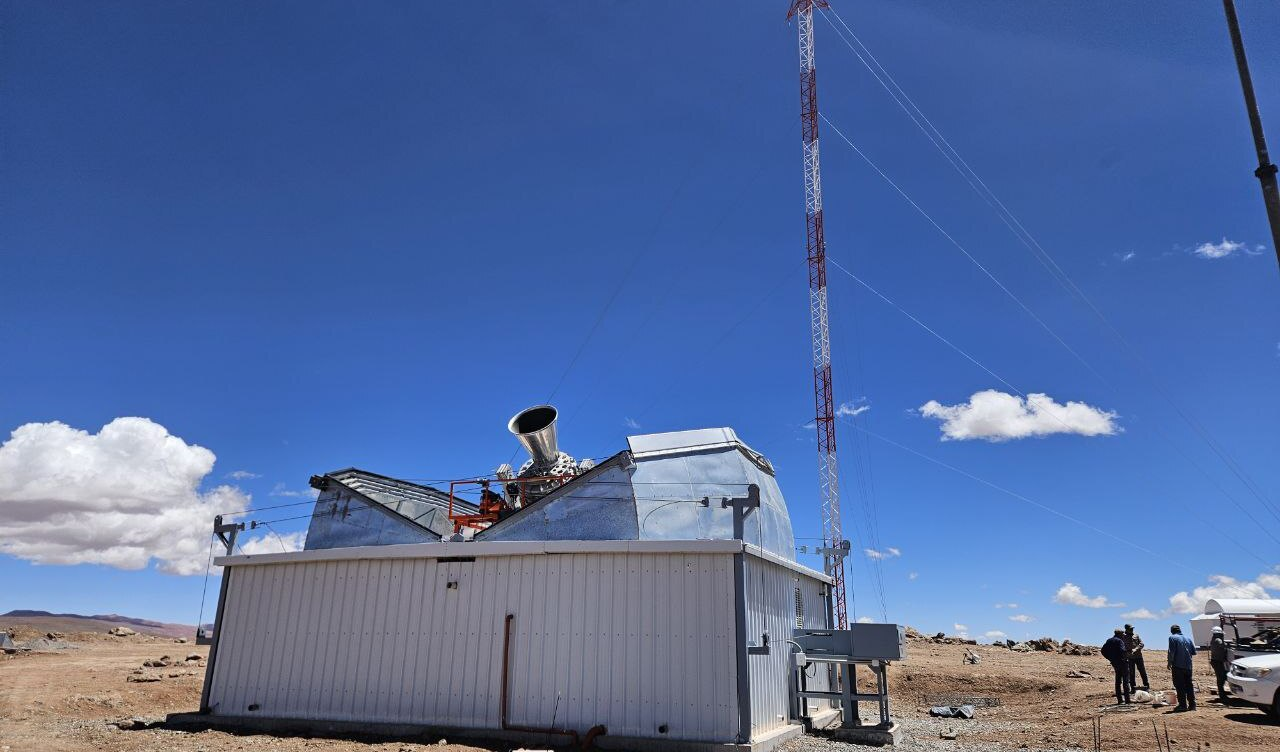
\includegraphics[width=0.9\linewidth]{qubic/qubic_cupula_r17.jpg}\\[2pt]
      \begin{tikzpicture}
        \node[inner sep=0pt, anchor=south west] (a) at (0,0)
          {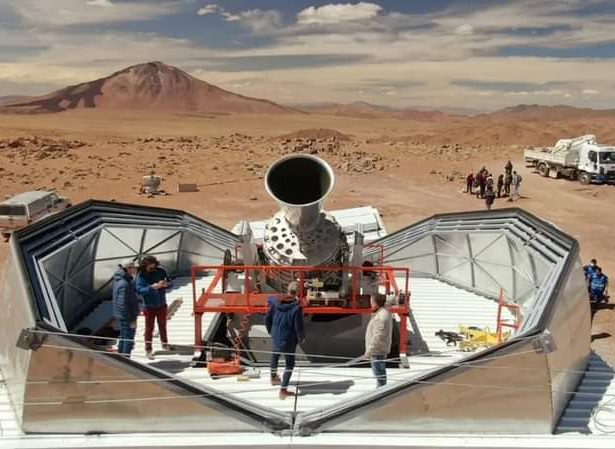
\includegraphics[width=0.445\linewidth]{qubic/qubic_e2_cupula_abierta_r.jpg}};
        \node[inner sep=0pt, anchor=south west] (b) at ([xshift=2pt]a.south east)
          {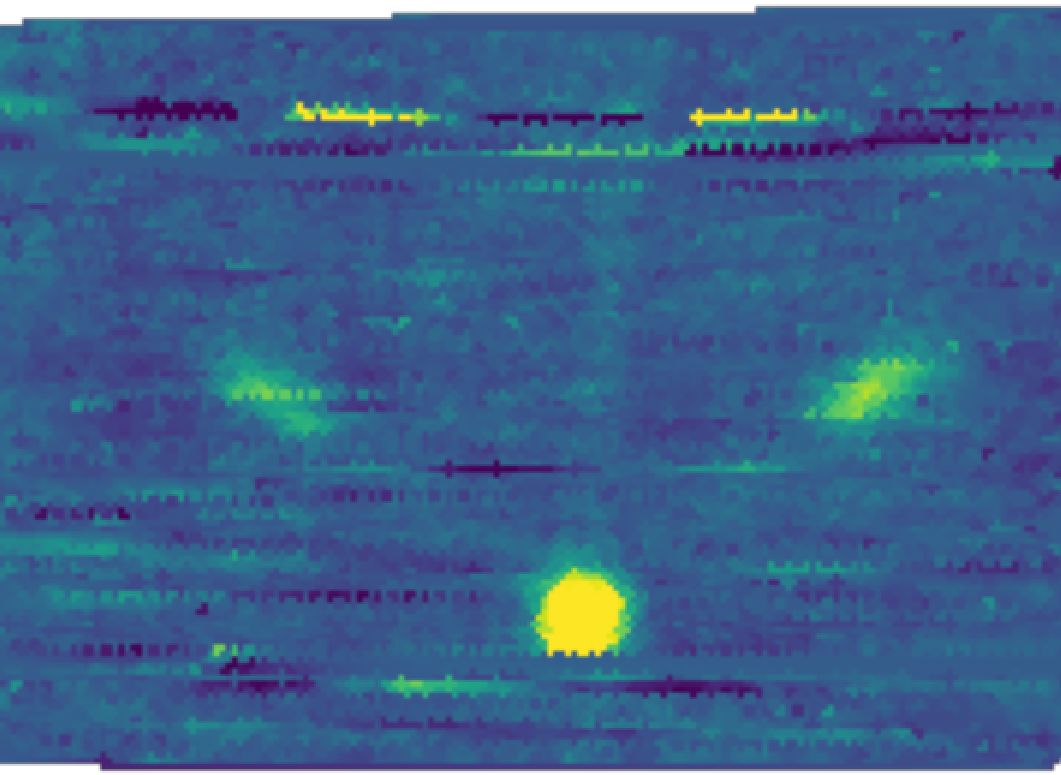
\includegraphics[width=0.445\linewidth]{qubic/qubic_luna_2026_r.png}};
        \node[anchor=south east, font=\tiny, text=white, fill=black, fill opacity=0.55,
          text opacity=1, inner sep=1.5pt] at (b.south east) {Luna, 11/03/2026};
      \end{tikzpicture}
    \column{0.53\textwidth}
      \small
      \textbf{Q\&U Bolometric Interferometer for Cosmology}: busca los modos B
      primordiales a 150 y 220\,GHz.
      \begin{itemize}\footnotesize
        \item \textbf{Alto Chorrillos}, cerca de San Antonio de los Cobres. El
          vapor de agua absorbe microondas: a esa altura el aire es muy seco.
        \item Seis países: Argentina, Francia, Irlanda, Italia, Reino Unido y EE.\,UU.
        \item \textbf{ITeDA}: infraestructura y montura, análisis de datos,
          nuevos sensores.
      \end{itemize}
      \vspace{3pt}
      \begin{tikzpicture}[x=1cm]
        \draw[itedaGray, thick] (-0.2,0) -- (7.6,0);
        \foreach \x/\y/\t in {0.2/2021/{llega a\\Salta}, 1.75/2022/{instalación\\en el sitio},
          3.3/2024/{torre de\\calibración}, 4.85/2025/{montura\\completa}, 6.6/2026/{primer barrido\\de la Luna}}{
          \fill[itedaOrange] (\x,0) circle (2.2pt);
          \node[font=\scriptsize\bfseries, above] at (\x,0.05) {\y};
          \node[font=\tiny, below, align=center] at (\x,-0.05) {\t};}
      \end{tikzpicture}
  \end{columns}
  \creditoizq{Fotos: F.~Sánchez, CLAF--CNRS (abr.\ 2026); L.~Silva Pizzi, Final de Estructura de la Materia 2 (2026)}
\end{frame}

% ---------------------------------------------------------------- 10
\begin{frame}{El desafío: una parte en cien millones}
  \begin{columns}[c,onlytextwidth]
    \column{0.47\textwidth}
    \begin{tikzpicture}
      \begin{loglogaxis}[coloquio, width=\linewidth, height=5.6cm,
        xmin=2, xmax=2500, ymin=0.005, ymax=200,
        xlabel={multipolo $\ell$}, ylabel={amplitud [$\mu$K]},
        xtick={10,100,1000}, xticklabels={10,100,1000},
        ytick={0.01,0.1,1,10,100}, yticklabels={{0,01},{0,1},1,10,100},
        grid=major]
        \fill[itedaOrange!14] (axis cs:30,0.005) rectangle (axis cs:200,200);
        \addplot[thick, cmbRojo] table[x=ell, y expr=sqrt(\thisrow{TT})] {data/planck_theory.dat};
        \addplot[thick, itedaTeal] table[x=ell, y expr=sqrt(\thisrow{EE})] {data/planck_theory.dat};
        \addplot[thick, violetaNu] table[x=ell, y expr=sqrt(\thisrow{BB})] {data/planck_theory.dat};
        \draw[violetaNu, dashed, thick] (axis cs:20,0.03) -- (axis cs:300,0.03);
        \node[font=\scriptsize, text=violetaNu, anchor=south, align=center]
          at (axis cs:7,0.012) {B primordiales:\\decenas de nK};
        \node[font=\scriptsize\bfseries, text=itedaOrange, anchor=north] at (axis cs:78,160) {QUBIC};
        \node[font=\scriptsize\bfseries, text=cmbRojo, anchor=south west] at (axis cs:2.3,70) {temperatura};
        \node[font=\scriptsize\bfseries, text=itedaTeal] at (axis cs:900,12) {E};
        \node[font=\scriptsize\bfseries, text=violetaNu, anchor=north] at (axis cs:1300,0.2) {B (lente)};
      \end{loglogaxis}
    \end{tikzpicture}
    \column{0.50\textwidth}
      \begin{columns}[T,onlytextwidth]
        \column{0.5\linewidth}
          \cifra{$10^{-8}$}{señal buscada respecto\\de lo que llega}\\[6pt]
          \cifra{$\sim$$10^{9}$}{fotones del CMB por\\segundo en cada detector}
        \column{0.5\linewidth}
          \cifra{0,6\,meV}{energía de cada fotón\\(3000 veces menos que el visible)}\\[6pt]
          \cifra{$10^{-20}$\,W}{diferencia de potencia\\a distinguir}
      \end{columns}
      \vspace{6pt}
      \begin{clave}
        No se cuentan fotones: se mide \textbf{potencia}, con miles de
        detectores muy fríos y años de integración.
      \end{clave}
  \end{columns}
  \credito{Espectros: Planck 2018, mejor ajuste $\Lambda$CDM (sin componente tensorial)}
\end{frame}

% ---------------------------------------------------------------- 11
\begin{frame}{Bolómetros y sensores de borde de transición (TES)}
  \begin{columns}[c,onlytextwidth]
    \column{0.45\textwidth}
      \centering
      \begin{tikzpicture}[x=0.8cm,y=0.8cm]
        \fill[pattern=north east lines, pattern color=itedaGray] (-0.4,-0.55) rectangle (4.4,-0.2);
        \draw[itedaGray, thick] (-0.4,-0.2) -- (4.4,-0.2);
        \node[font=\scriptsize, anchor=north] at (2,-0.6) {baño frío a $\approx$0,3\,K};
        \draw[decorate, decoration={zigzag, amplitude=1.2mm, segment length=2.2mm},
          thick, itedaTeal] (2,-0.2) -- (2,1.2);
        \node[font=\scriptsize, anchor=west, text=itedaTeal, align=left] at (2.25,0.5)
          {vínculo térmico\\débil};
        \draw[thick, fill=itedaOrange!25, rounded corners=1pt] (0.6,1.2) rectangle (3.4,2.0);
        \node[font=\scriptsize] at (1.85,1.6) {absorbente};
        \fill[itedaTealDark] (3.0,1.32) rectangle (3.32,1.48);
        \draw[itedaTealDark] (3.16,1.48) -- (3.9,2.2) node[above, font=\scriptsize] {TES};
        \draw[foton, itedaOrange, thick] (0.4,3.1) -- (1.2,2.1);
        \draw[foton, itedaOrange, thick] (1.5,3.2) -- (1.9,2.1);
        \node[font=\scriptsize, text=itedaOrange, anchor=south] at (0.9,3.15) {luz del cielo};
      \end{tikzpicture}\\[6pt]
      \footnotesize
      \textbf{Bolómetro}: la luz \textbf{calienta} un absorbente unido
      débilmente a un baño frío. Cuánto se calienta mide la potencia.
    \column{0.52\textwidth}
      \begin{tikzpicture}
        \begin{axis}[coloquio, width=\linewidth, height=3.6cm,
          xmin=395, xmax=425, ymin=-0.05, ymax=1.15,
          xlabel={temperatura del sensor [mK]}, ylabel={resistencia},
          grid=major, ytick=\empty]
          \addplot[very thick, itedaTeal, domain=395:425, samples=150]
            {0.5*(1+tanh((x-410)/2.2))};
          \fill[itedaOrange] (axis cs:410.6,0.635) circle (2.5pt);
          \node[font=\scriptsize, text=itedaOrange, anchor=west, align=left]
            at (axis cs:411.8,0.45) {punto de\\operación};
          \node[font=\scriptsize, anchor=south] at (axis cs:401,0.04) {superconductor};
          \node[font=\scriptsize, anchor=north] at (axis cs:420,0.97) {normal};
          \node[font=\scriptsize, text=itedaGray, anchor=south east] at (axis cs:409.5,0.75)
            {$T_c\approx410$\,mK};
        \end{axis}
      \end{tikzpicture}
      \begin{clave}
        \textbf{TES}: un superconductor operado justo \textbf{en su
        transición}, donde la resistencia cambia violentamente con la
        temperatura: un calentamiento ínfimo se vuelve un cambio grande de
        corriente.
      \end{clave}
  \end{columns}
  \creditoizq{Curva ilustrativa. $T_c$ (NbSi): QUBIC IV, arXiv:2101.06787}
\end{frame}

% ---------------------------------------------------------------- 12
\begin{frame}{Cómo se lee un TES: el SQUID}
  \centering
  \begin{tikzpicture}[x=1cm,y=1cm,
    caja/.style={rounded corners=3pt, draw=itedaTeal, fill=itedaLight, thick,
      minimum height=1.2cm, text width=2.15cm, align=center, font=\scriptsize},
    clave/.style={caja, draw=itedaOrange, fill=itedaOrange!12},
    paso/.style={-{Stealth[length=2.4mm]}, very thick, itedaOrange}]
    \node[caja] (luz) at (0,0) {\textbf{Luz del cielo}\\llega más o menos potencia};
    \node[caja] (tes) at (2.9,0) {\textbf{TES}\\se calienta y cambia su resistencia};
    \node[caja] (bob) at (5.8,0) {\textbf{Bobina}\\cambia la corriente y su campo};
    \node[clave] (sq) at (8.7,0) {\textbf{SQUID}\\cambia el flujo y su tensión};
    \node[caja] (asic) at (11.6,0) {\textbf{Electrónica}\\a 40\,K: amplifica y digitaliza};
    \draw[paso] (luz) -- (tes); \draw[paso] (tes) -- (bob);
    \draw[paso] (bob) -- (sq); \draw[paso] (sq) -- (asic);
    \node[font=\tiny, text=itedaGray, below=1pt of tes] {0,3\,K};
    \node[font=\tiny, text=itedaGray, below=1pt of sq] {1\,K};
  \end{tikzpicture}\\[6pt]
  \begin{columns}[c,onlytextwidth]
    \column{0.30\textwidth}
      \centering
      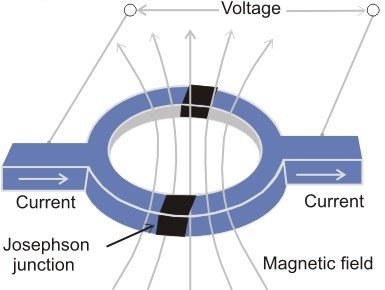
\includegraphics[width=0.72\linewidth]{qubic/squid_e2_esquema.jpg}\\[0pt]
      {\tiny Anillo con dos junturas Josephson}
    \column{0.67\textwidth}
      \footnotesize
      \begin{itemize}\footnotesize
        \item \textbf{Juntura Josephson}: barrera aislante finísima entre dos
          superconductores, que la corriente cruza por \textbf{efecto túnel}.
        \item La corriente se divide en dos ramas; el flujo magnético del
          anillo las \textbf{desfasa} y al juntarse \textbf{interfieren}, como
          en una doble rendija.
      \end{itemize}
      \begin{clave}
        La tensión oscila con período $\Phi_0=h/2e$ (\textbf{cuanto de flujo}):
        un cambio minúsculo de corriente se vuelve medible.
        \textbf{El TES mide, el SQUID lee.}
      \end{clave}

  \end{columns}
\end{frame}

% ---------------------------------------------------------------- 13
\begin{frame}{¿Por qué el detector está más frío que el CMB?}
  \begin{columns}[c,onlytextwidth]
    \column{0.64\textwidth}
      \centering
      \begin{tikzpicture}[x=1cm,y=1cm]
        % termómetro horizontal, escala log: x = 2*log10(T/0.1 K)
        \shade[left color=cmbAzul!70, right color=cmbRojo!70, rounded corners=4pt]
          (0,0) rectangle (7.0,0.35);
        \foreach \t/\x/\l/\c/\up in {
            300/6.95/{300 K\\ambiente}/itedaGray/1,
            77/5.77/{77 K\\nitrógeno líquido}/itedaGray/0,
            4.2/3.25/{4 K\\helio líquido}/itedaGray/1,
            2.725/2.87/{2,7 K\\\textbf{CMB}}/itedaOrange/0,
            0.3/0.95/{0,3 K\\\textbf{detectores}}/itedaTeal/1}{
          \draw[\c, very thick] (\x,-0.05) -- (\x,0.4);
          \ifnum\up=1
            \node[font=\scriptsize, text=\c, align=center, anchor=south] at (\x,0.45) {\l};
          \else
            \node[font=\scriptsize, text=\c, align=center, anchor=north] at (\x,-0.1) {\l};
          \fi}
      \end{tikzpicture}\\[8pt]
      \begin{minipage}{0.96\linewidth}
      \footnotesize
      La temperatura de 2,7\,K describe el \textbf{espectro} de la luz
      (cuánta energía trae), no la temperatura a la que debe estar el
      detector. Hay que enfriarlo porque:
      \begin{enumerate}\footnotesize
        \item el \textbf{ruido térmico} del propio sensor baja con la temperatura;
        \item todo lo que está caliente \textbf{brilla} en microondas: lentes,
          espejos y paredes se enfrían para no tapar al cielo;
        \item la \textbf{transición superconductora} del TES está a $\sim$0,4\,K.
      \end{enumerate}
      \end{minipage}
    \column{0.33\textwidth}
      \centering
      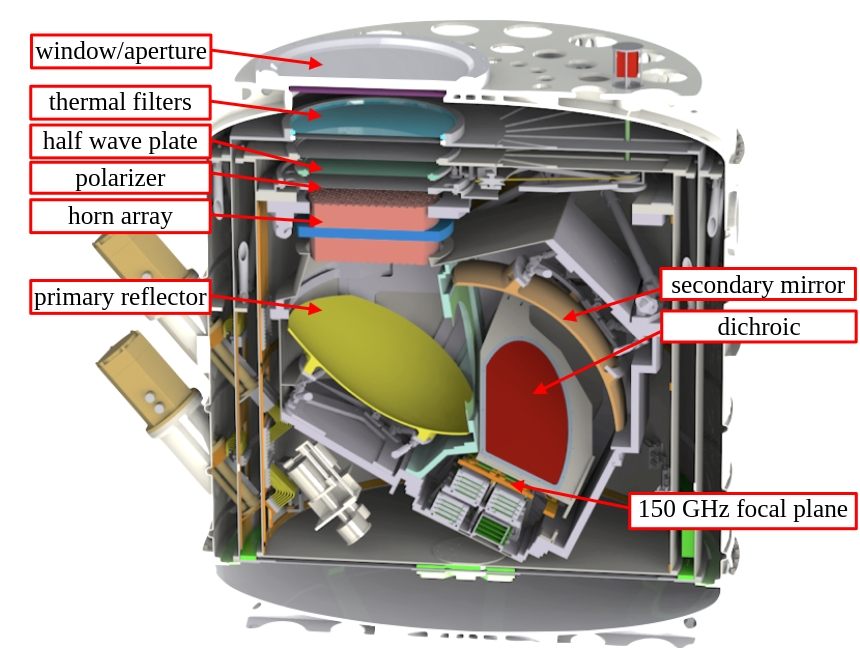
\includegraphics[width=0.7\linewidth]{qubic/qubic_criostato_corte.jpg}\\[2pt]
      {\scriptsize Criostato de QUBIC (1,8\,m $\times$ 1,6\,m): etapas a 40\,K,
      4\,K, 1\,K y 0,3\,K}\\[6pt]
      \begin{clave}
        Un termómetro al sol no está a 5800\,K: \textbf{mide la potencia}
        que le llega.
      \end{clave}
  \end{columns}
  \creditoizq{Corte del criostato: Colaboración QUBIC (vía F.~Sánchez, 2026)}
\end{frame}

% ---------------------------------------------------------------- separador
\bloque{}
\begin{frame}[plain]
  \fondo[0.15]{halzen/cielo_montanas.jpg}
  \velo[0.8]{l}
  \begin{tikzpicture}[remember picture, overlay]
    \node[anchor=west, text=white, align=left, text width=10cm]
      at ([xshift=0.9cm]current page.west) {%
      {\small\color{itedaOrange}\bfseries DE LA LUZ MÁS ANTIGUA\\A LAS PARTÍCULAS MÁS ENERGÉTICAS}\\[8pt]
      {\fontsize{34}{38}\selectfont\bfseries Rayos cósmicos}\\[8pt]
      {\normalsize Aceleradores naturales, el espectro\\y el Observatorio Pierre Auger}};
  \end{tikzpicture}
  \creditoblanco{Foto: vía F.~Halzen, Erice 2024}
\end{frame}
